\documentclass{beamer}

\usepackage[utf8]{inputenc}
\usepackage[T1]{fontenc}
\usepackage[francais]{babel}

\usetheme{Darmstadt}
\usecolortheme{seahorse}

\usepackage{graphicx}
\input{/home/pablo/Documents/Examples/lstset}

\AtBeginSection[]{
    \begin{frame}
        \frametitle{Plan}
        \tableofcontents[currentsection,hideothersubsections]
    \end{frame} 
}

\titlegraphic{
    \begin{columns}
        \column{.15\textwidth}
        
\includegraphics[width=\textwidth]{img/imag.eps}
        \column{.45\textwidth}
        
\includegraphics[width=\textwidth]{img/topSolid.eps}
    \end{columns}
}

\title{Projet TopSolid}
\author{Ariane Lefebvre \and Sina Miladi \and Pablo Coves}
\date{}

\begin{document}
\maketitle

\section{Description du projet}
\subsection{Missler}
\begin{frame}
    \frametitle{TopSolid}
    \begin{columns}
        \column{.5\textwidth}
        \begin{itemize}
            \item Première apparition avec le logiciel TopCAD en 1987.
            \item Ensemble de logiciels dédiés à la CFAO et ERP.\\
            \item Solution pour la conception et la fabrication de pièces ou outils.
            \item Permet le pilotage de machine outils et le suivi des produits.
        \end{itemize}
        \column{.5\textwidth}
        \begin{figure}
            
\includegraphics[width=\textwidth]{img/topSolid.jpg}
            \caption{TopSolid Galaxy}
            \label{TopSolid}
        \end{figure}
    \end{columns}
\end{frame}
\subsection{Mots clés}
\begin{frame}
    \begin{columns}
        \column{.5\textwidth}
        \frametitle{Une scène}
        Une scène est composée de plusieurs éléments:
        \begin{itemize}
            \item Une matrice:\\
                Définie par un polygone, fixe au cours du temps.
            \item Un poinçon:\\
                Défini par un polygone dont on connait le mouvement au cours du temps.
            \item Une tôle:\\
                Considérée d'épaisseur fixe, elle est décrite par sa fibre neutre.
        \end{itemize}
        \column{0.5\textwidth}
        \begin{figure}
            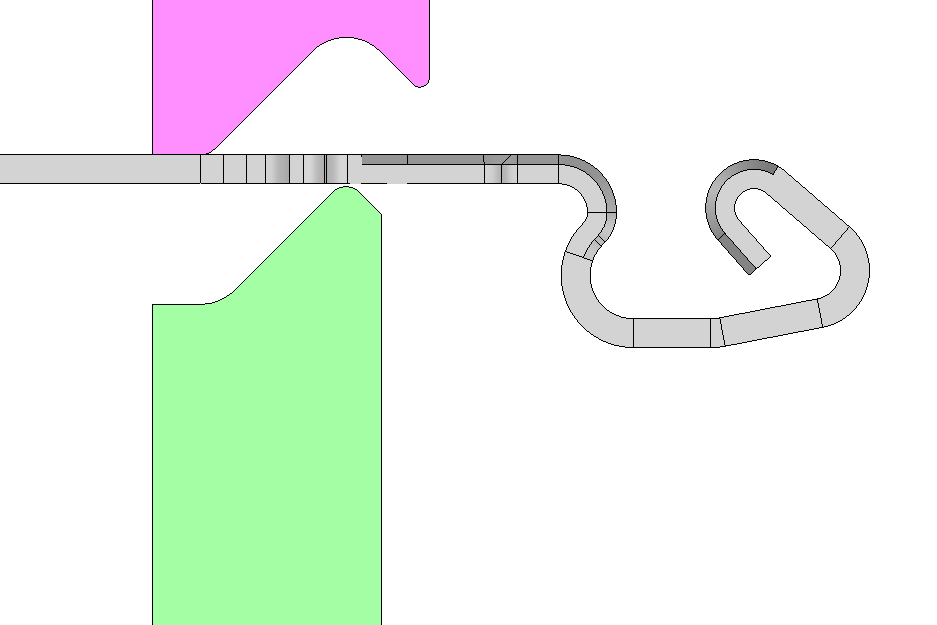
\includegraphics[width=\textwidth]{img/fibreNeutre.jpg}
            \caption{Fibre neutre}
            \label{FibreNeudre}
        \end{figure}
    \end{columns}
\end{frame}
\begin{frame}
    \frametitle{Une étape}
    \begin{columns}
        \column{.7\textwidth}
        Chaque position du poinçon correspond à une étape d'une scène.\\
        Il faut prendre en compte:
        \begin{itemize}
            \item Les forces appliquées sur la tôle.
            \item Le déplacement induit par ces forces.
            \item Le retour élastique lors du retrait du poinçon.
        \end{itemize}
        \column{.3\textwidth}
        \begin{figure}
            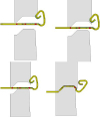
\includegraphics[width=\textwidth]{img/etape.jpg}
            \caption{Étapes}
            \label{Étape}
        \end{figure}
    \end{columns}
\end{frame}
\begin{frame}
    \frametitle{Fichier de scène}
    \begin{itemize}
        \item Utilisation du XML: facile à lire et à faire évoluer.
        \item Un fichier de scène est utilisé pour décrire les différents éléments d'une scène.
            \begin{itemize}
                \item Forme et position de la matrice.
                \item Forme, position et déplacements restants du poinçon.
                \item Forme et épaisseur de la tôle.
            \end{itemize}
        \item Format aussi utilisé pour sauvegarder l'état du système à chaque étape.
    \end{itemize}
\end{frame}

\section{Description du logiciel}
\subsection{Freefem++}
\begin{frame}
    \frametitle{Gestion de la déformation}
    \begin{columns}
        \column{.5\textwidth}
        Un logiciel de résolution d'équations différentielles par élément finis.\\
        Il est utilisé pour:
        \begin{itemize}
            \item Générer un maillage pour la représentation.
            \item Calculer le déformation de la tôle selon les forces appliquées.
        \end{itemize}
        \column{.5\textwidth}
        \begin{figure}
            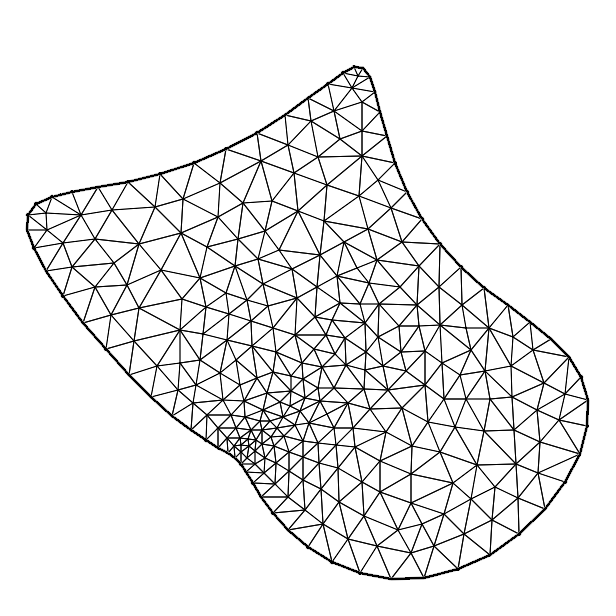
\includegraphics[width=\textwidth]{img/maillage.png}
            \caption{Exemple de maillage}
            \label{Maillage}
        \end{figure}
    \end{columns}
\end{frame}
\subsection{Interface utilisateur}
\begin{frame}
    \frametitle{La fenêtre}
    \framesubtitle{Aperçu}
    \begin{columns}
        \column{.5\textwidth}
        \begin{itemize}
            \item Une zone centrale de visualisation.
                \begin{itemize}
                    \item Scène en mouvement.
                    \item Barre d'actions.
                \end{itemize}
            \item Une zone latérale d'options.
                \begin{itemize}
                    \item Pas de déplacement.
                    \item Temps de visualisation.
                \end{itemize}
        \end{itemize}
        \column{.5\textwidth}
        \begin{figure}
            %TODO: mettre image de la fenêtre.
            %\includegraphics[width=\textwidth]{img/fenetre.jpg}
            %\caption{}
            \label{Fenetre}
        \end{figure}
    \end{columns}
\end{frame}
\begin{frame}
    \frametitle{La fenêtre}
    \framesubtitle{Zone de rendu}
    \begin{itemize}
        \item QGLWidget.
        \item Interaction à la souris: sélection des points à suivre.
        \item Affichage en transparence de l'aire couverte couverte par la tôle durant la scène complète.
    \end{itemize}
\end{frame}
\begin{frame}
    \frametitle{Pour un rendu réaliste}
    \framesubtitle{Calcul de la position du poinçon}
    \begin{center}
        $P(t) = \frac{-Dmax}{2}*\cos(\frac{2}{Tmax}*\pi*t)+\frac{Dmax}{2}$
    \end{center}
        \begin{figure}
            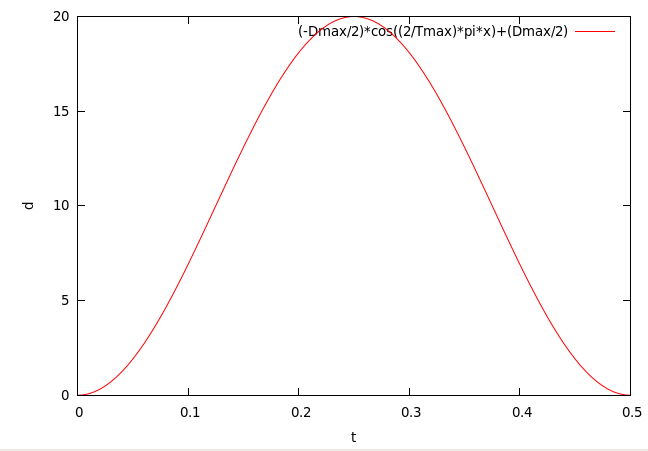
\includegraphics[width=.7\textwidth]{img/position.png}
            \caption{Position du poinçon}
            \label{Position}
        \end{figure}
\end{frame}
\begin{frame}
    \frametitle{Pour un rendu réaliste}
    \framesubtitle{Calcul de la vitesse du poinçon}
    \begin{center}
        $V(t) = \frac{\pi*Dmax}{Tmax}*\sin(\frac{2*\pi}{Tmax}*t)$
    \end{center}
    \begin{figure}
        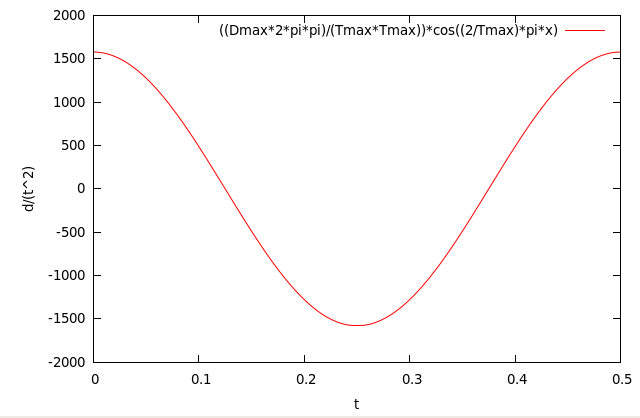
\includegraphics[width=.7\textwidth]{img/acceleration.png}
        \caption{Vitesse du poinçon}
        \label{Vitesse}
    \end{figure}
\end{frame}
\begin{frame}
    \frametitle{Pour un rendu réaliste}
    \framesubtitle{Calcul de l'accélération du poinçon}
    \begin{center}
        $A(t) = \frac{2*\pi^2*Dmax}{Tmax^2}*\cos(\frac{2*\pi}{Tmax}*t)$
    \end{center}
        \begin{figure}
            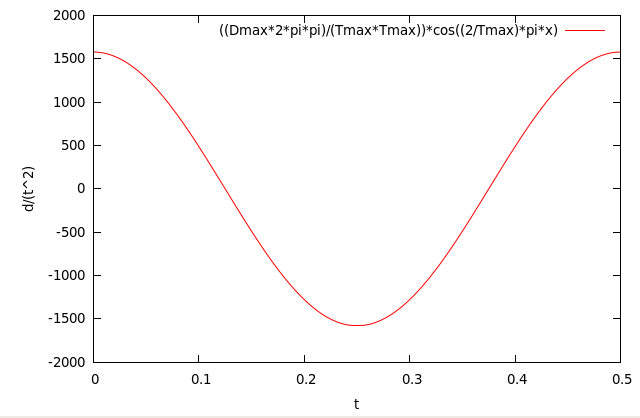
\includegraphics[width=.7\textwidth]{img/acceleration.png}
            \caption{Accélération du poinçon}
            \label{Accélération}
        \end{figure}
\end{frame}
\begin{frame}
    \frametitle{Pour un rendu réaliste}
    \framesubtitle{Calcul des forces sur la tôle}
\end{frame}

\section{Organisation}
\subsection{Répartition des tâches}
\begin{frame}
    \begin{itemize}
        \item MCS: utilisation de freefem++.\\
            Gestion de la déformation de la tôle à chaque étape.
        \item ICAO: rendu graphique des scènes.\\
        Interface utilisateur et intéractions souris.
        \item ICAO: gestion des fichiers et parseurs XML.\\
            Communication avec freefem++.
    \end{itemize}
\end{frame}
\subsection{Diagramme de Gantt}

\section{Conclusion}
\subsection{Perspectives}
\begin{frame}
    \begin{itemize}
        \item Intégration au logiciel TopSolid.
        \item Modification de l'épaisseur de la tôle.
        \item Modification du poinçon et de la matrice par l'utilisateur.
    \end{itemize}
\end{frame}
\subsection{Questions}
\begin{frame}
    Merci de votre écoute.
    \begin{figure}
        
\includegraphics[width=.55\textwidth]{img/conclusion.png}
        %\caption{}
        \label{Conclusion}
    \end{figure}
    \hfill Des questions?
\end{frame}

\end{document}
